\section{\texttt{\CiT} System Overview}\label{sec:overview}



\begin{figure*}[b]
\vspace{-4mm}
\centering 	
 		{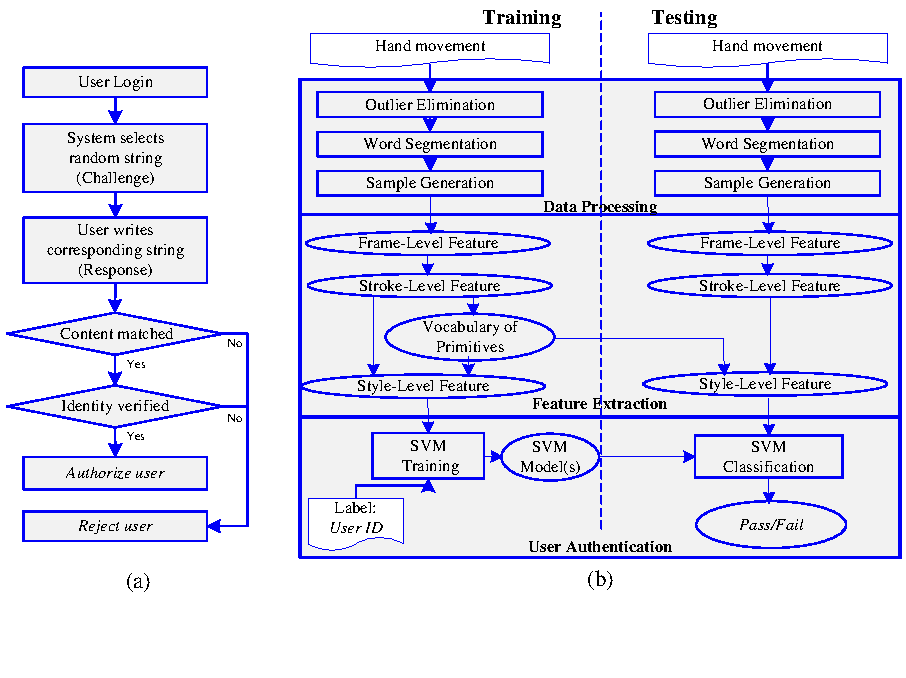
\includegraphics[width=2.0\columnwidth]{./Graphic/SystemFlow/SystemFlow_all_ccs_2017_style.pdf}}
\vspace{-18mm}
  \caption{\jing{(a) Flow chart of \CiT system. 
  (b) Flow chart of identity matching. 
  Details of the 3-Level feature extraction are shown in Figure~\ref{fig:featureFlow}.}
  \vspace{-3mm}
  }
  \label{fig:sysFlow}
\end{figure*}

\subsection{{Why does \CiT work?}}
%\subsection{Characterize Handwriting Styles} 

The \CiT system consists of two steps: verifying whether what a user writes matches what is asked for, and verifies the identity of the user. \jingap{
The first step is not the focus of this paper and can be accomplished by utilizing the prior work explained in Section~\ref{sec:related}.  
In particular, the user writes the content that the system provides (the Challenge). After receiving the input from the user (the Response), the system checks if the input content is the same as the system expected. As such, an attacker cannot simply `replay' handwriting performed in the past by a legitimate user. Based on the assumption that the replay attack would not be an issue for \CiT, 
}
%rely on existing technologies~\cite{ICDAR15:OnlineHandwriting,LeeV12Cursive,Madhvanath2012,Plamondon2000Review}, 
 we focus on the second step: how to verify users based on their handwriting styles, i.e., based on \textit{how} they write instead of \textit{what} they write. The challenges are to correctly recognize a user even if he/she writes different contents, and to distinguish users even if they write the same content. The difficulties stem from the possibility of handwriting variation (especially in writing different contents) of the same user and occasional handwriting similarity (especially in writing the same content) between different users.  The key to overcome the challenges is to characterize handwriting styles effectively and efficiently. 

\emph{Stroke Segments for Effective Modeling.} The model characterizing handwriting styles has to be content-independent. A naive approach could be to extract fingertip trajectories that represent each individual character and then to group the ones of the same characters for further comparison. However, such a method may be overkill, as the handwriting in the 3D space is difficult to be delimited precisely, as shown in \figref{fig:dataWords3user}. 
Although content recognition is possible, perfectly delimiting the fingertip trajectory of each letter is challenging. To avoid the burden of extracting individual symbols, we choose to characterize handwriting styles 
by short-length continuous trajectories, which are analogous to strokes~\cite{Component94,word-seg-stroke}. In practice, it is difficult to accurately divide a handwriting trajectory into meaningful strokes with variable lengths. We simply divide fingertip trajectories into a set of short, fixed-length \emph{stroke segments}. To reduce the impact of the starting point on a trajectory for stroke segment partition, we apply a temporal-sliding window over the fingertip trajectory for constructing stroke segment, and the constructed stroke segments can be partially overlapped.


Stroke segments can be considered as the basic building blocks that compose symbols. Although the underlying content in fingertip trajectories may be different, some characters may share similar stroke segments. Thus, the two fingertip trajectories created by the same user when writing different sets of words could contain a large percentage of the similar stroke segments. The stroke segments belonging to different users typically show little similarity.  For instance,  as shown in \figref{fig:bphmn}, the letters \texttt{b} and \texttt{p} have similar composition.
%, so do the letters `n' and `h'.  
Some stroke segments (denoted by different colors on the characters) of \texttt{b} and \texttt{p} from the same user show similarity, but the Stroke segments of User 1 are different from the ones of User 2. Thus, it is imaginable that the trajectories of the word \texttt{`bob'} and \texttt{`pop'} from the same user may have many similar stroke segments, but the ones from different users may share few similar stroke segments.


\emph{Vocabulary for Improving Efficiency.}
We define a \textit{frame} on a trajectory as a fingertip position, and consider the associated coordinates and kinematic features at each frame: \textit{frame-level features}. To compare the similarity between stroke segments, we can concatenate the frame-level features of all frames of a stroke segment to form \textit{stroke segment-level features}. Then,
we can combine all the stroke segment-level features of a trajectory sample to construct one \textit{style-level feature}, which is the unit to represent the handwriting style.  However, simply combining all the stroke segment-level features will lead to high-dimensional vectors. % and irregularized feature vectors.
To address this issue, we can define a stroke segment vocabulary that best represents the collection of stroke segments of all the enrolled users. The vocabulary consists of a set of primitives corresponding to typical stroke segments of those users, and each primitive will be assigned a unique index. The creation of a vocabulary can be conducted during the training phase. During the testing stage, each stroke segment is assigned the index of its nearest primitive. This way we reduce each high-dimensional stroke segment-level features to an integer index. 


Finally, to compare the similarity between handwriting styles of multiple samples, we perform statistical analysis to achieve content-independence.  Specifically, we obtain statistics on the stroke segment indices within a trajectory sample for constructing a low-dimensional feature for a sample. \jingap{Instead of using the histogram or probability density functions (PDFs) of the individual stroke segment indices~\cite{He:ICDAR15:PolarStroke, 
Bulacu07text-independentwriter, Li2007:StrokeProbabilityDistribution}}, we examine the temporal transition between stroke segments. The intuition is that a user may tend to write the same sequence of stroke segments, and such a sequence may be essential to represent handwriting styles. Concretely, we construct a co-occurrence matrix that counts the number of occurrences of each possible stroke segment (index) transition between temporally adjacent stroke segment pairs. This co-occurrence matrix reflects the distribution of the temporal stroke segment transition and we reshape it into a vector as a feature vector of a sample.




\begin{figure}[!b]
\vspace{-8mm}
\centering
\begin{tabular}{c}
{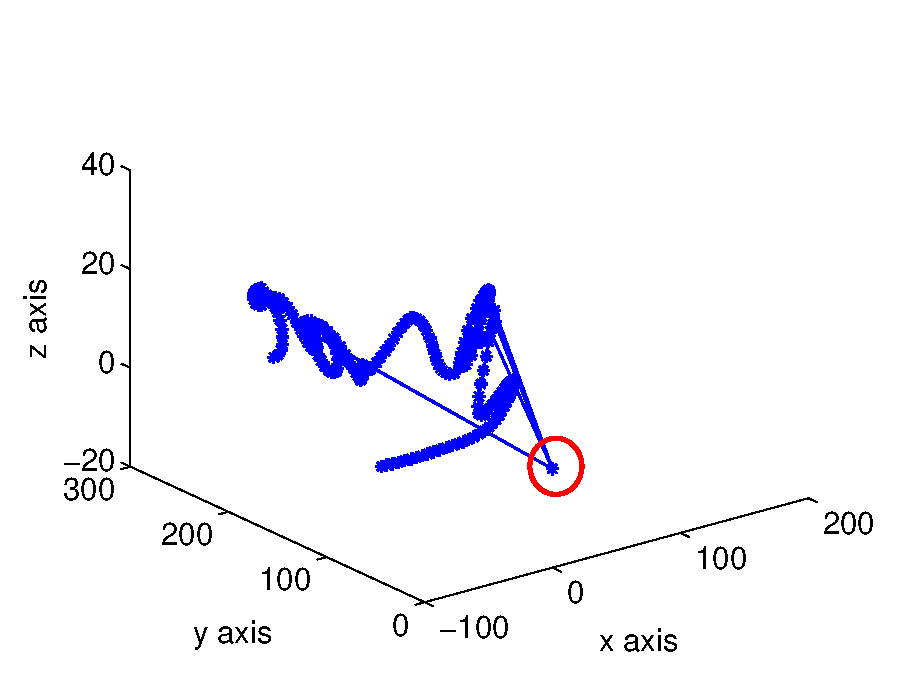
\includegraphics[width=0.65\columnwidth]{./Graphic/noise/noise_1.eps}} 
% &
%{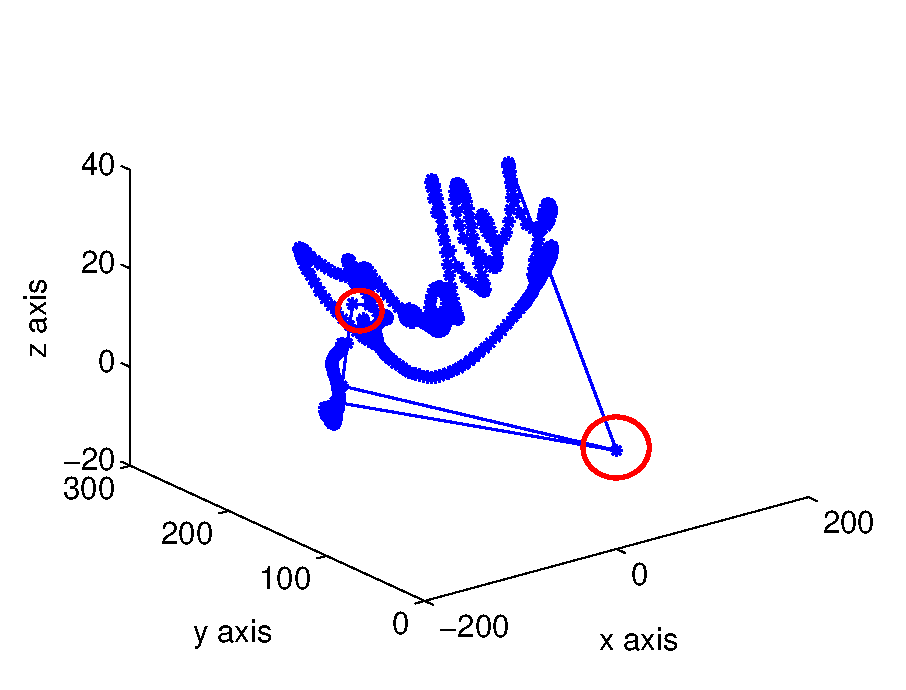
\includegraphics[width=0.53\columnwidth]{./Graphic/noise/noise_2.eps}}  &
%{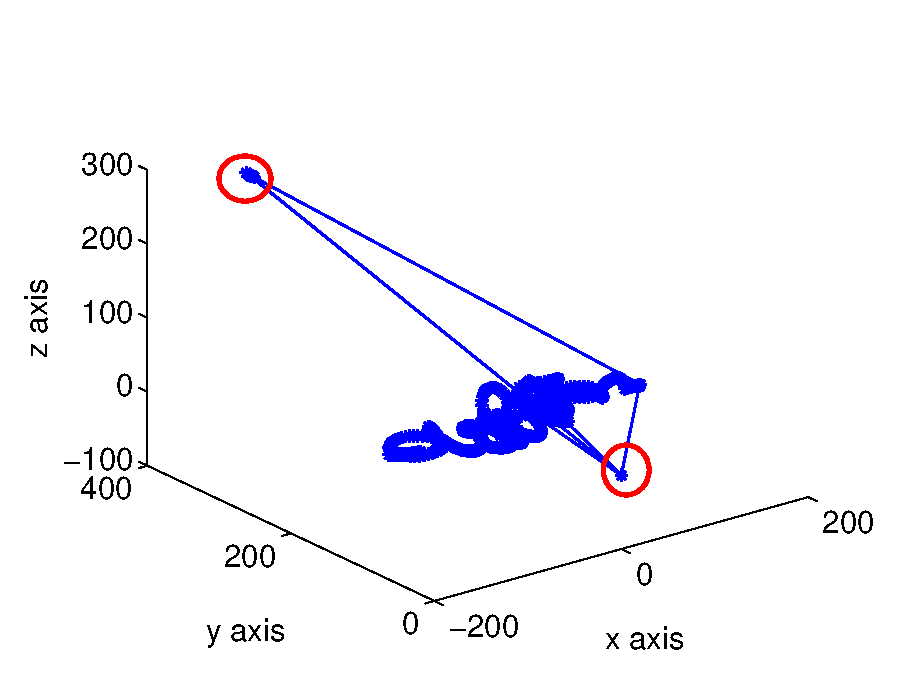
\includegraphics[width=0.53\columnwidth]{./Graphic/noise/noise_3.eps}}
\end{tabular}
\vspace{-2mm}
\caption{An illustration of the outliers in Leap Motion data. The red circles highlight the frames with outliers.}
\label{fig:noises}
\end{figure}




Continue with the example in \figref{fig:bphmn}, $50$ primitives were derived to form a vocabulary for illustration. We observe that the similar letter sets (e.g., \texttt{b} and \texttt{p}) written by the same user contain similar stroke segment indices and transition pattern of stroke segment indices, while the stroke segment sequences of the same letter (e.g., \texttt{b} or \texttt{p}) written by different users share few similarities.  
%In particular, we notice that the index sequence of character `b' and `p' written by the same subject show strong similarity, while the same characters written by different users exhibit difference. 
This example encourages us to study the effectiveness of using vocabulary and transition between stroke segments to model the handwriting style. 

\subsection{{How does \CiT work?}}
%\subsection{System Overview}



The \CiT system consists of a Leap Motion for capturing fingertip movements in the 3D space, computing and storage units for challenge-response processing and identity authentication. \figref{fig:sysFlow}(a) shows a the flow chart of the challenge-response authentication. 

The \CiT authentication process consists of two phases: enrollment and testing. During an enrollment, the system will capture the initial handwriting and create an account for a user. These handwriting inputs will be used for training. In a testing phase, the system first select a random string. After capturing the user's writing movements, the system first performs a content check, i.e., verifying whether what a user writes matches the random string, and then tests the user's identity.  \figref{fig:sysFlow} illustrates a detailed flow chart of identity matching. 

\jingap{
\emph{Content Matching.} 
The focus of this paper is to study the biometric built on handwriting motion instead of content check, because several literatures can achieve the content check, as shown in Section~\ref{sec:related}. Therefore, we do not include the technique details of this part in the paper. } 

%Spatial Features : Trajectory formation Normalization to  fixed center of gravity for the system.

%In addition, since our handwriting data is written in the air, we can project the 3D writings into its main plane (a 2D plane). 
%We briefly overview the biometric-related processes in this section and postpone the detailed discussion to Section~\ref{sec:data} and ~\ref{sec:feature}.  
%Note that our system can perform a content check to detect such scenarios, i.e., utilizing similarity comparison or content recognition using online handwritng recognition techniques~\cite{Tappert90}.  


\emph{Data Processing.} Both training and testing phases require data processing and feature extraction. The goal of data processing is to prepare the raw motion data captured by Leap Motion and generate a handwriting sample, which consists of a number of frames that represent the motion of the fingertip. 
The data processing will remove outliers and meaningless transition trajectories from the data,  as well as partition the handwriting trajectory into samples, on which the features can be calculated to represent the writing style. 


\emph{Feature Extraction.} After data processing, a \CiT system extracts three levels of features from each sample: frame-level features, stroke segment-level features, and style-level features. Level by level, the \CiT system is able to derive features that effectively and efficiently model the handwriting styles of users. 

\emph{SVM Training and Testing.}
In \figref{fig:sysFlow}, \CiT system uses the extracted style-level features for both classifier training and testing. The classifier has to achieve two goals: correctly authenticate a legitimate user and reject any impostors that are not part of the pool. %This maps to the scenario of teleconference, whereby the system tries to identify whether the comments are entered by one of the attendees or by an attacker. 







